%%%%%%%%%%%%%%%%%%%%%%%%%%%%
%Capstone Proposal for Udacity - Juan Jos� Madrigal
%%%%%%%%%%%%%%%%%%%%%%%%%%%%

%%%%%% Packages

\documentclass[11pt]{article}
\usepackage[latin1]{inputenc}
\usepackage{graphicx}
\usepackage{hyperref}
\usepackage[none]{hyphenat}
\hypersetup{colorlinks,urlcolor=light,citecolor=light}
\usepackage{multicol}
\usepackage{array}
\usepackage{cancel}
\usepackage{color}
\usepackage{amssymb}
\usepackage{amsopn}
\usepackage{amsmath}
\usepackage{enumitem}
\usepackage[default,osfigures,scale=0.95]{opensans}
\setlength{\hoffset}{-1.85cm}
\setlength{\voffset}{-2.5cm}
\setlength{\textwidth}{469pt}
\setlength{\textheight}{640pt}
\setlength{\parindent}{0cm}
\definecolor{dark}{rgb}{0.15,0.30,0.4}
\definecolor{light}{rgb}{0.15,0.3,0.6}

%%%%%% Document

\begin{document}
	
	%%% Header
	
	\begin{center}
		{{\Large\textsc{\color{dark}Machine Learning Engineer Nanodegree}}}\\
		\vspace{0.3cm}
		{{\LARGE\textsc{\color{dark}Capstone Proposal}}}
	\end{center}
	
	\vspace{-0.4cm}
	
	\textcolor{dark}{\rule{\textwidth}{3pt}}
	
	%%% Personal data
	
	\begin{minipage}[t]{7cm}
		\flushleft
		Juan Jos� Madrigal Mart�nez\\
		January 30, 2017\\
	\end{minipage}
	\hfill
	%%% Contact
	\begin{minipage}[t]{7cm}
		\flushright
		Madrid, Spain\\
		(+0034) 600 86 32 48\\
		juanjomadrigal326@gmail.com\\
		\href{https://es.linkedin.com/in/juan-jose-madrigal}{LinkedIn} \quad
		\href{https://github.com/jxm-math}{GitHub} \quad
		\href{https://www.kaggle.com/jxmmath}{Kaggle} \quad
		\href{https://discussions.udacity.com/users/juanjo_madrigal/summary}{Udacity}
	\end{minipage}\\\\
	
	\vspace{0.3cm}

%%% Domain Background

{{\Large\textsc{\color{dark}Domain Background}}}

\vspace{-0.25cm}

\textcolor{dark}{\rule{\linewidth}{2pt}} \vspace{-0.5cm}

% (approx. 1-2 paragraphs)

This project aims at building a video analysis system for surveillance purposes. It basically finds and indexes the movement events filmed by a fixed camera.\\

Video surveillance has become a major and widely used tool for multiple issues \cite{video_surveillance} and is supported by many companies \cite{video_surveillance_company_1} \cite{video_surveillance_company_2}. But the huge ammount of information which is usually dealt with has led to the need to use Machine Learning techniques to extract patterns, predictions and other refined information. This approach is being implemented \cite{ml_company_1} and there is much work for Machine Learning engineers to do in this field. \\

An efficient implementation of Machine Learning techniques to video surveillance would prevent users from dealing with a sequential (and manual) search through the (perhaps many hours long) video source, which is rather inefficient, boring and error prone, thus providing a major tool for a wide range of purposes.

\begingroup
\renewcommand{\section}[2]{}%
\begin{thebibliography}{}
	\bibitem{video_surveillance}
	\href{https://en.wikipedia.org/wiki/Surveillance#Cameras}{Wikipedia - Surveillance / Cameras}
	
	\bibitem{video_surveillance_company_1}
	\href{https://www.videosurveillance.com/}{VideoSurveillance.com}
	
	\bibitem{video_surveillance_company_2}
	\href{http://www.tyco.com/}{Tyco}
	
	\bibitem{ml_company_1}
	\href{http://briefcam.com/}{Briefcam}
	
\end{thebibliography}
\endgroup

%In this section, provide brief details on the background information of the domain from which the project is proposed. Historical information relevant to the project should be included. It should be clear how or why a problem in the domain can or should be solved. Related academic research should be appropriately cited in this section, including why that research is relevant. Additionally, a discussion of your personal motivation for investigating a particular problem in the domain is encouraged but not required.\\

%%% Problem Statement

{{\Large\textsc{\color{dark}Problem Statement}}}

\vspace{-0.25cm}

\textcolor{dark}{\rule{\linewidth}{2pt}} \vspace{-0.5cm}

% (approx. 1 paragraph)

To apply unsupervised Machine Learning clustering algorithms to detect and quantify the movement events filmed by a fixed camera. The algorithms are to be applied to a tridimensional binary array obtained from the original video after some careful video-preprocessing (see below). Further refinements may also be tackled, such as finding time-parametric curves accurately fitting each movement event. \\

%In this section, clearly describe the problem that is to be solved. The problem described should be well defined and should have at least one relevant potential solution. Additionally, describe the problem thoroughly such that it is clear that the problem is quantifiable (the problem can be expressed in mathematical or logical terms) , measurable (the problem can be measured by some metric and clearly observed), and replicable (the problem can be reproduced and occurs more than once).\\

%%% Datasets and Inputs

{{\Large\textsc{\color{dark}Datasets and Inputs}}}

\vspace{-0.25cm}

\textcolor{dark}{\rule{\linewidth}{2pt}} \vspace{-0.5cm}

% (approx. 2-3 paragraphs)

The datasets and inputs for this project will be obtained after some video preprocessing made on sample videos. The selected videos are located in \href{https://github.com/jxm-math/capstone_project/tree/master/data/unprocessed_videos}{capstone\_project/data/unprocessed\_videos} and they have been downloaded from \href{http://www.viratdata.org/}{VIRAT Video Dataset} \cite{virat}. The video preprocessing is carried out using the free packages \href{http://scikit-image.org/}{SciKitImage} and \href{http://www.scikit-video.org/}{SciKitVideo} and has been generously provided by \href{http://wardenautomation.com/}{WardenAutomation}.\\

The video preprocessing takes as input a \texttt{.avi} $\texttt{M}\times \texttt{N}$ pixels video and a \texttt{.png} $\texttt{M}\times \texttt{N}$ pixels picture (\textit{background}). For each frame in the video, the frame and the background are compared pixel-wise, and the difference is recorded in a $\texttt{M}\times \texttt{N}$ binary array, where $1$ denotes difference (above some threshold) and $0$ denotes no difference.

\begin{center}
	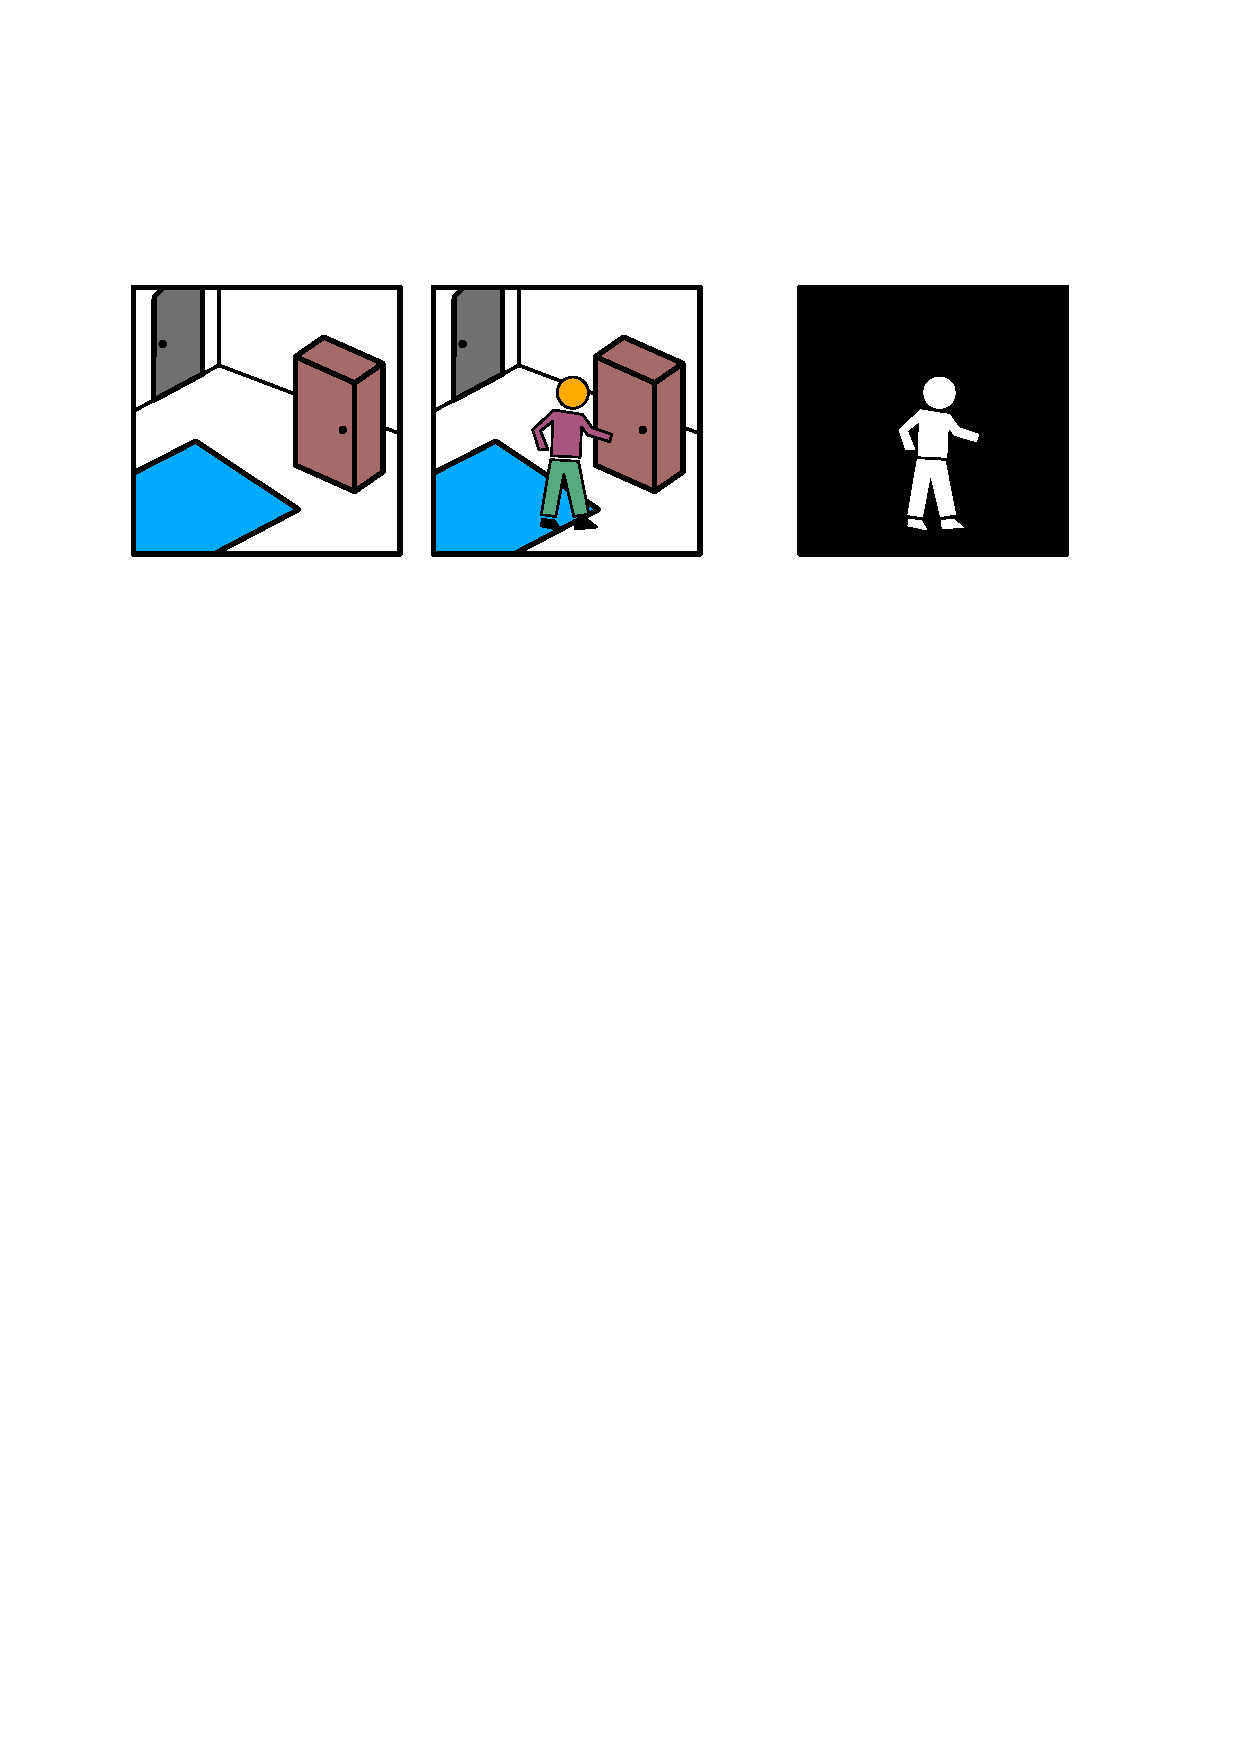
\includegraphics[scale=1]{cpj_1.pdf}
\end{center}

If the video has $\texttt{T}$ frames, then the video preprocessing gives as output a $\texttt{M}\times \texttt{N}\times \texttt{T}$ binary array, which is supposed to capture the movement in our scene and that will be the primary input for the project. These arrays are saved not as arrays as such but as \texttt{.avi} files, and are located in \href{https://github.com/jxm-math/capstone_project/tree/master/data/processed_videos}{capstone\_project/data/processed\_videos}.\\

\begin{center}
	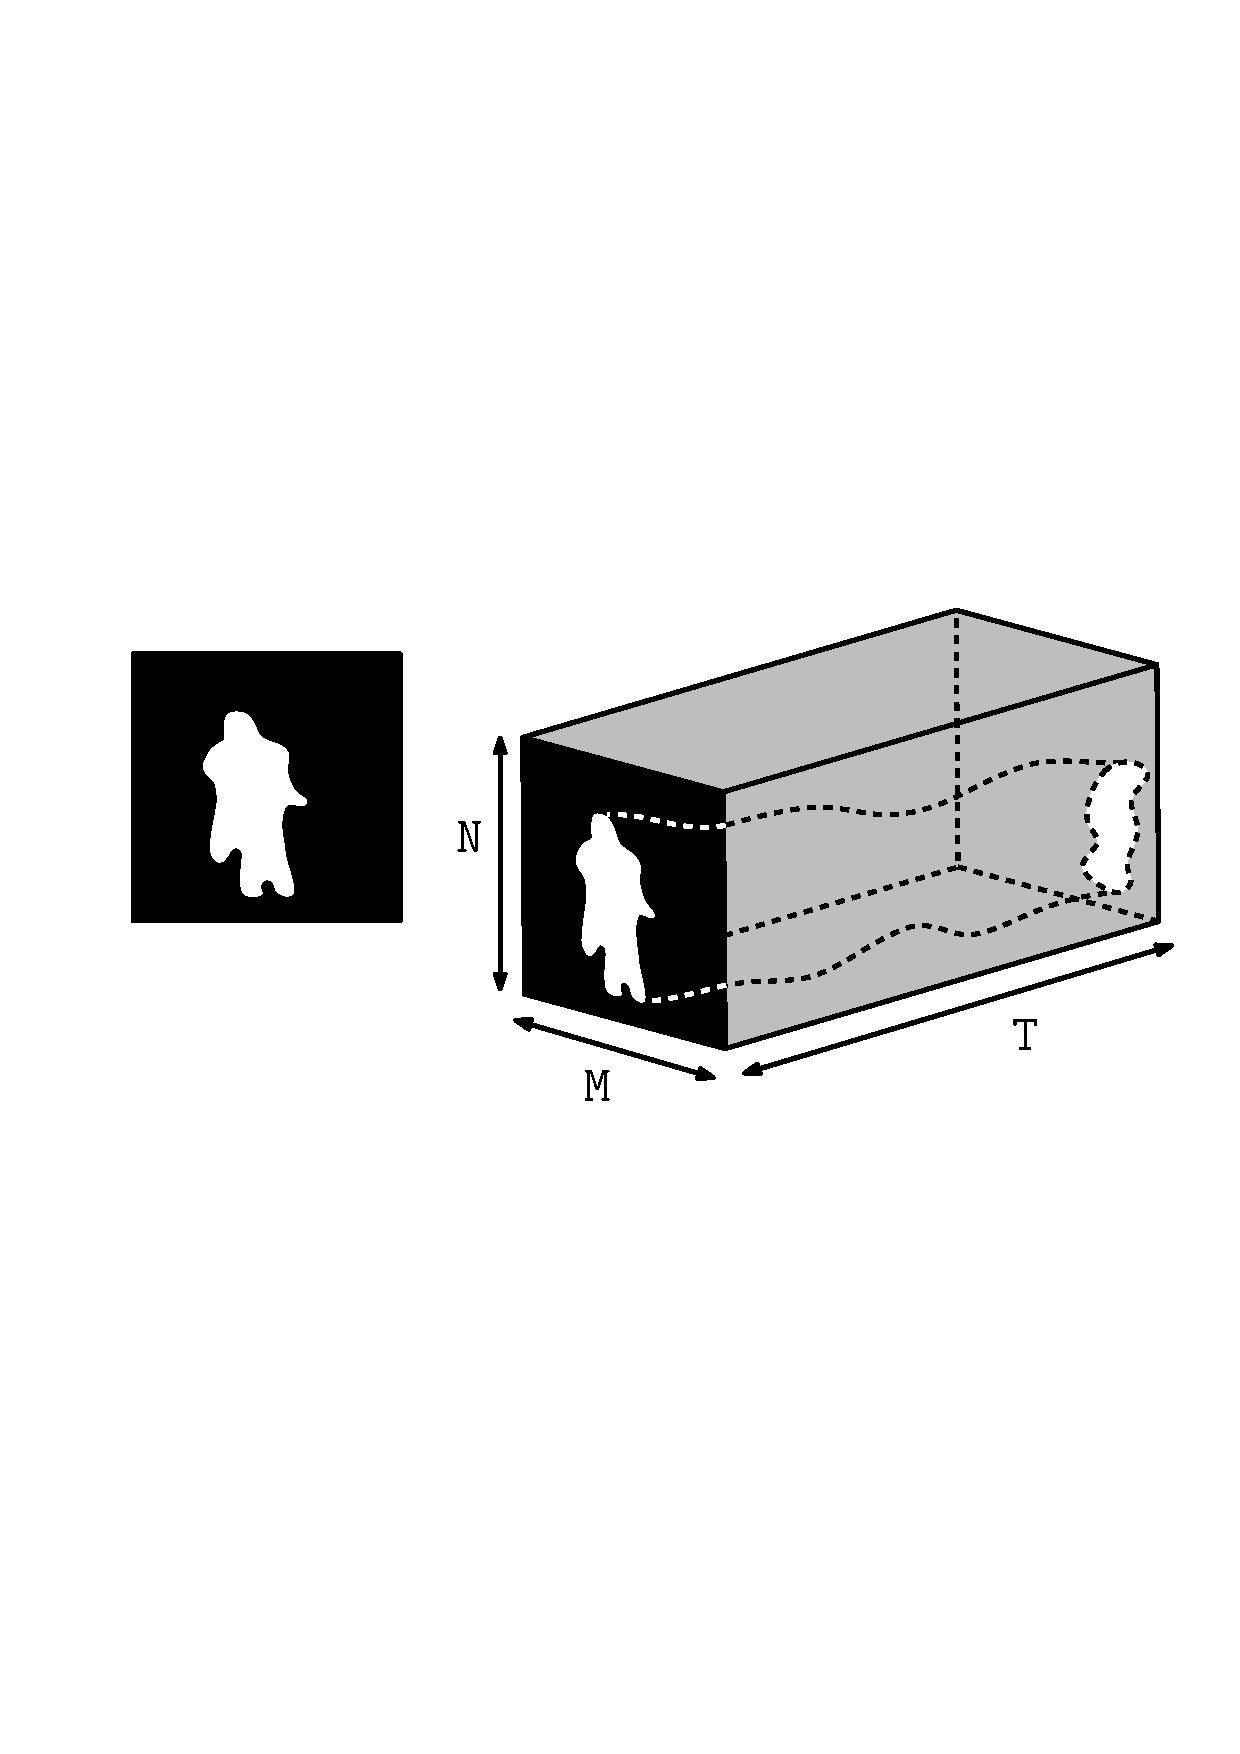
\includegraphics[scale=0.8]{cpj_2.pdf}
\end{center}

The total ammount of data in this latter folder sums up to 10 videos (and a exploratory \texttt{video1.avi}) whose duration ranges between half and three minutes. This should be enough to tune our algorithm (see below) for the purposes of similar (fixed-camera) videos.

\begingroup
\renewcommand{\section}[2]{}%
\begin{thebibliography}{}
	\bibitem{virat}
	\textbf{A Large-scale Benchmark Dataset for Event Recognition in Surveillance Video}, Sangmin Oh, Anthony Hoogs, Amitha Perera, Naresh Cuntoor, Chia-Chih Chen, Jong Taek Lee, Saurajit Mukherjee, J.K. Aggarwal, Hyungtae Lee, Larry Davis, Eran Swears, Xiaoyang Wang, Qiang Ji, Kishore Reddy, Mubarak Shah, Carl Vondrick, Hamed Pirsiavash, Deva Ramanan, Jenny Yuen, Antonio Torralba, Bi Song, Anesco Fong, Amit Roy-Chowdhury, and Mita Desai, \textit{Proceedings of IEEE Comptuer Vision and Pattern Recognition (CVPR), 2011}.
\end{thebibliography}
\endgroup

%In this section, the dataset(s) and/or input(s) being considered for the project should be thoroughly described, such as how they relate to the problem and why they should be used. Information such as how the dataset or input is (was) obtained, and the characteristics of the dataset or input, should be included with relevant references and citations as necessary It should be clear how the dataset(s) or input(s) will be used in the project and whether their use is appropriate given the context of the problem.\\

%%% Solution Statement

{{\Large\textsc{\color{dark}Solution Statement}}}

\vspace{-0.25cm}

\textcolor{dark}{\rule{\linewidth}{2pt}} \vspace{-0.5cm}

% (approx. 1 paragraph)

We propose the use of \href{http://scikit-learn.org/stable/modules/clustering.html#dbscan}{DBSCAN clustering algorithm}, which is implemented in \href{http://scikit-learn.org/}{SciKitLearn}. This clustering algorithm is well-suited for our generic clusters, which are uneven in size and non-convex.\\

DBSCAN clustering algorithm (\textit{Density-based spatial clustering of applications with noise}) takes primarily two parameters

\begin{itemize}
	\item \texttt{min\_samples}, integer
	\item \texttt{eps}, float
\end{itemize}

and classifies the points in a metric space into three groups

\begin{itemize}
	\item \textbf{Core points}: points whose \texttt{eps}-neighbourhood contains at least \texttt{min\_samples} points
	\item \textbf{Reachable points}: points that are not core points themselves, but that cointain some core point in their \texttt{eps}-neighbourhood
	\item \textbf{Outliers or noise}: points that are not core points nor reachable points
\end{itemize}

\begin{center}
	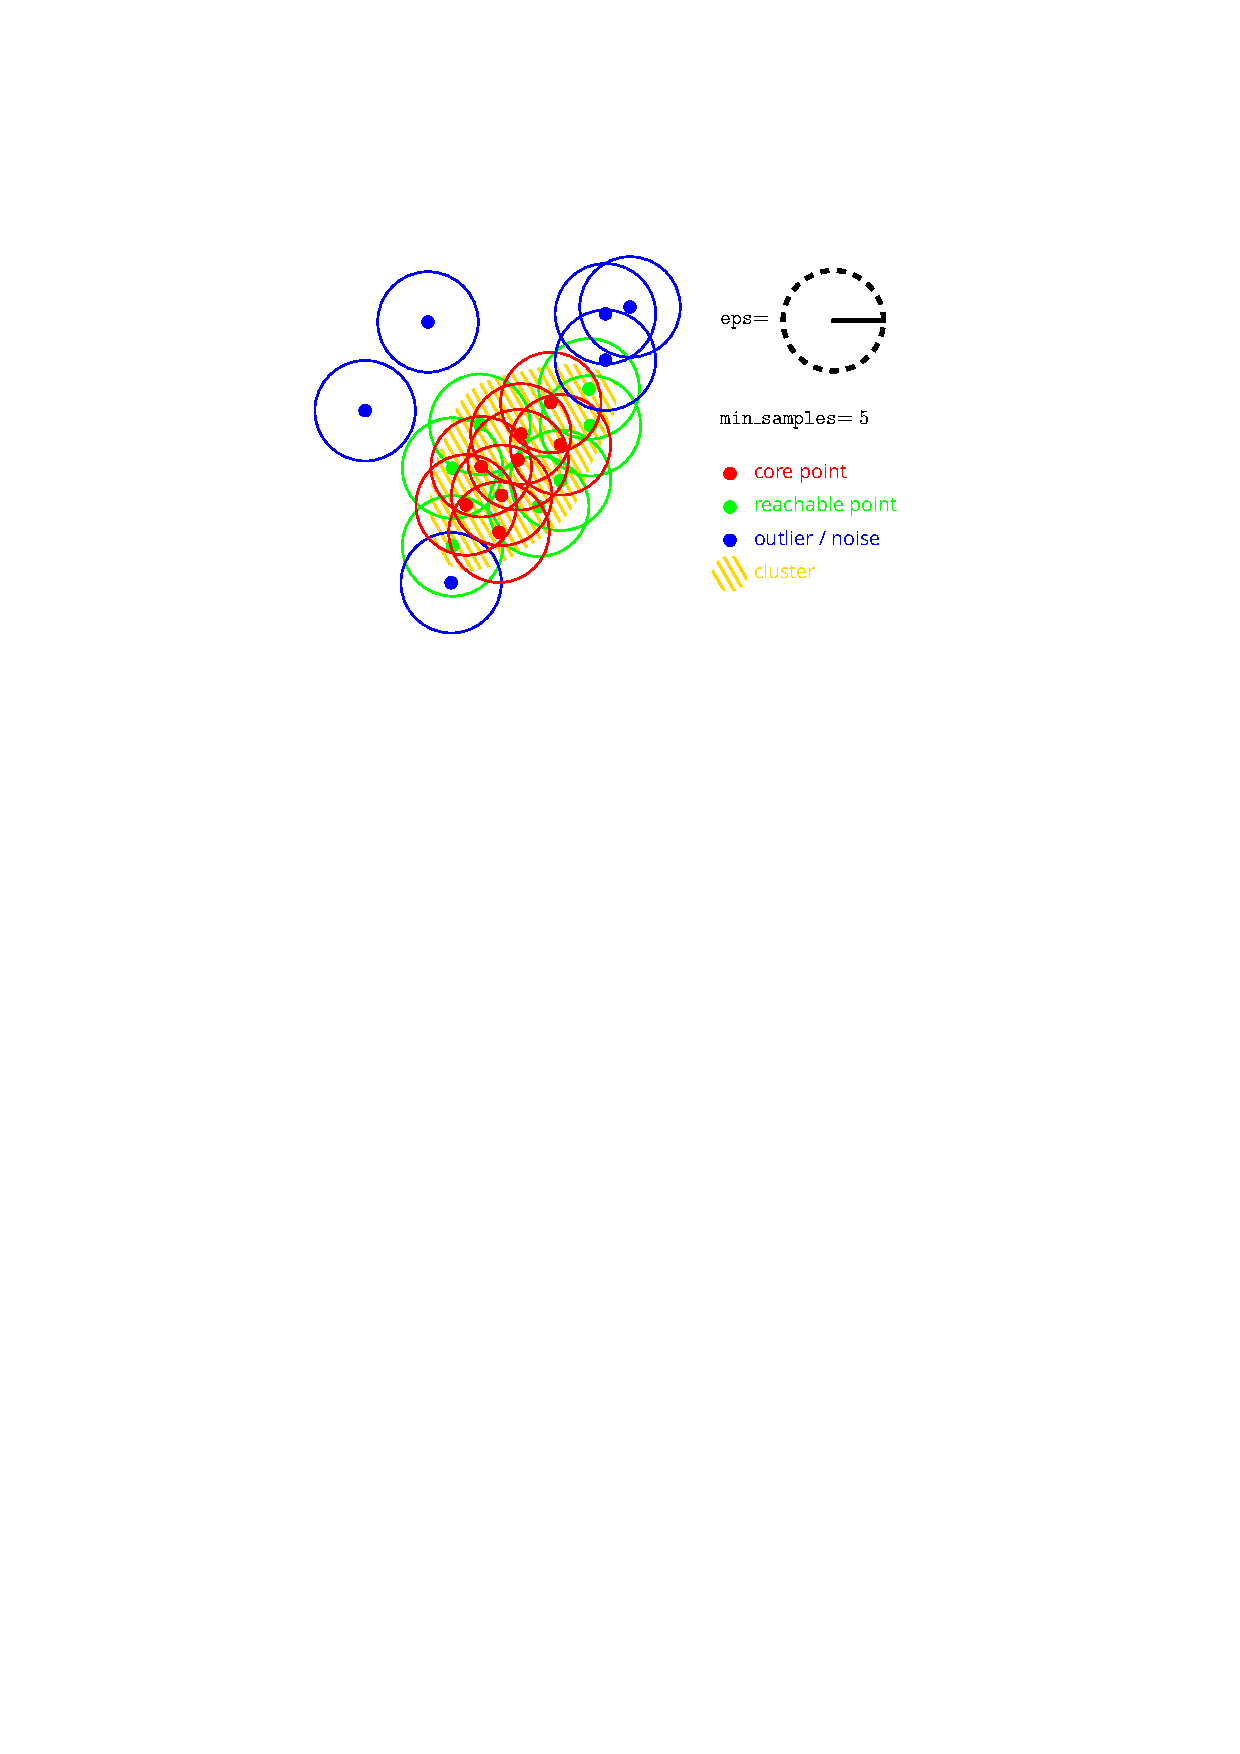
\includegraphics[scale=1.2]{dbscan_illustration.pdf}
\end{center}

Each group of mutually \texttt{eps}-path-connected core points with the associated reachable points forms a cluster. The way in which the algorithm is implemented may lead to some indeterminisms, such as reachable points reached from two different clusters, but the number of clusters and their intrinsic shape are well-determined.\\

This algorithm has some major advantages that make it well-suited for our clustering problem:

\begin{itemize}
	\item The number of expected clusters is not to be specified. This is crucial, since our goal is to determine the number of clusters / movement-events
	\item The clusters may be of any shape
	\item The algorithm deals well with noise (our arrays, generated from video processing, always have noise)
\end{itemize} 

\begingroup
\renewcommand{\section}[2]{}%
\begin{thebibliography}{}
	\bibitem{dbscan_wikipedia}
	\href{https://en.wikipedia.org/wiki/DBSCAN}{DBScan - Wikipedia}
\end{thebibliography}
\endgroup

%In this section, clearly describe a solution to the problem. The solution should be applicable to the project domain and appropriate for the dataset(s) or input(s) given. Additionally, describe the solution thoroughly such that it is clear that the solution is quantifiable (the solution can be expressed in mathematical or logical terms) , measurable (the solution can be measured by some metric and clearly observed), and replicable (the solution can be reproduced and occurs more than once).\\


%%% Benchmark Model

{{\Large\textsc{\color{dark}Benchmark Model}}}

\vspace{-0.25cm}

\textcolor{dark}{\rule{\linewidth}{2pt}} \vspace{-0.5cm}

% (approximately 1-2 paragraphs)

A major Benchmark Model may be found at \href{http://www.wisdom.weizmann.ac.il/~vision/VideoAnalysis/Demos/SpaceTimeActions/SpaceTimeActions_pami07.pdf}{Actions as Space-Time Shapes}.\\

This work deals with the recognition of activities in a single movement-event. For this movement-event to be analysed, spectral clustering methods are used \cite{spectral_clustering_wikipedia}. The performance is measured in terms of misclassifications (2.17\%, 7.91\% and 36.40\% for different methods). 

\begingroup
\renewcommand{\section}[2]{}%
\begin{thebibliography}{}
	\bibitem{spectral_clustering_wikipedia}
	\href{https://en.wikipedia.org/wiki/Spectral_clustering}{Spectral Clustering - Wikipedia}
\end{thebibliography}
\endgroup

%In this section, provide the details for a benchmark model or result that relates to the domain, problem statement, and intended solution. Ideally, the benchmark model or result contextualizes existing methods or known information in the domain and problem given, which could then be objectively compared to the solution. Describe how the benchmark model or result is measurable (can be measured by some metric and clearly observed) with thorough detail.\\

%%% Evaluation Metrics

{{\Large\textsc{\color{dark}Evaluation Metrics}}}

\vspace{-0.25cm}

\textcolor{dark}{\rule{\linewidth}{2pt}} \vspace{-0.5cm}

% (approx. 1-2 paragraphs)

The direct metric to tune the main parameters of DBScan (\texttt{eps} and \texttt{min\_samples}) will be the Sum of Square Errors according to the expected value of clusters, which is known on beforehand for each of the training videos.\\

Once the algorithm is accurately tuned, the metric(s) used to estimate the quality of our clustering will comprise

\begin{itemize}
	\item Homogeneity
	\item Completeness
	\item V-measure
	\item Adjusted Rand Index
	\item Adjusted Mutual Information
	\item Silhouette Coefficient
\end{itemize} 

%In this section, propose at least one evaluation metric that can be used to quantify the performance of both the benchmark model and the solution model. The evaluation metric(s) you propose should be appropriate given the context of the data, the problem statement, and the intended solution. Describe how the evaluation metric(s) are derived and provide an example of their mathematical representations (if applicable). Complex evaluation metrics should be clearly defined and quantifiable (can be expressed in mathematical or logical terms).\\

%%% Project Design

{{\Large\textsc{\color{dark}Project Design}}}

\vspace{-0.25cm}

\textcolor{dark}{\rule{\linewidth}{2pt}} \vspace{-0.5cm}

% (approx. 1 page)

A theoretical workflow for approaching a solution would include

\begin{enumerate}
	\item To apply the video preprocessing techniques to the selected videos to get the tridimensional binary arrays, which are the main input for our Machine Learning work.
	\item To apply \href{http://scikit-learn.org/stable/modules/clustering.html#dbscan}{DBSCAN clustering algorithm} to each array for a first contact with the potential results.
	\item To compare the previous results with a manual detection and indexing for a small set of training videos. This may lead to a major refinement of the main algorithms. Together with this manual checking, the metrics mentioned above will be used and compared with the latter, thus finding which metrics work best for our video surveillance context.
	\item To apply the refined algorithms and selected metrics to a large variety of videos. Further tuning may be implemented. 
	\item To provide code for spatial visualisation of all the previous processes.
	\item From all the extracted data, to make conclussions about the success of our study and devise new ways or fields for further work.
\end{enumerate}

%In this final section, summarize a theoretical workflow for approaching a solution given the problem. Provide thorough discussion for what strategies you may consider employing, what analysis of the data might be required before being used, or which algorithms will be considered for your implementation. The workflow and discussion that you provide should align with the qualities of the previous sections. Additionally, you are encouraged to include small visualizations, pseudocode, or diagrams to aid in describing the project design, but it is not required. The discussion should clearly outline your intended workflow of the capstone project.\\



%Before submitting your proposal, ask yourself. . .

%Does the proposal you have written follow a well-organized structure similar to that of the project template?

%Is each section (particularly Solution Statement and Project Design) written in a clear, concise and specific fashion? Are there any ambiguous terms or phrases that need clarification?

%Would the intended audience of your project be able to understand your proposal?

%Have you properly proofread your proposal to assure there are minimal grammatical and spelling mistakes?

%Are all the resources used for this project correctly cited and referenced?
	
\end{document}
